\documentclass[12pt]{article}

\usepackage[hmargin=1in,vmargin=1in]{geometry}
\usepackage{parskip}
\usepackage{hyperref}
\usepackage{graphicx}
\usepackage{color}
\usepackage{verbatim}
\hypersetup{pdfstartview=FitV,hidelinks}



\begin{document}

{
  \Large
  \centering
  {\bf Lab 9 Assignment --- Distance Sampling} \\
  Due before your next lab \par
}

\vspace{10pt}

% Analysis of the (fake) Mongolian gazelle ({\it Procapra gutturosa})
% data using program DISTANCE.  

The purpose of this lab is to learn how to use program DISTANCE to
estimate abundance and density using distance sampling data. You will
do this by analyzing fake data on Mongolian gazelle ({\it Procapra
  gutturosa}). The data are fake, but they are based loosely on the
study that we discussed in lecture. Note that gazelles were detected
in groups (ie, herds), and the distance data are distances to group
centers. 

Put your answers in a Word file and upload it to ELC. Name the file
something like ``Chandler-lab9.docx''. Due before your next lab.  




%\clearpage

\section*{\large Part I: Format data and import into DISTANCE}



\begin{enumerate}
\item Open DISTANCE and create a new project by clicking
  \verb+File > New Project ...+. Name the project something like
  ``Gazelle.dst''  
    
  \item Use the ``New Project Setup Wizard'' and select the
    following options: 
  \begin{enumerate}
    \item Analyze a survey that has been completed
    \item Line transect, single observer, perpendicular distance,
      \textcolor{red}{clusters of objects} 
    \item Distance = Meter, transect length = Kilometers,
      \textcolor{red}{area = Square kilometer}
    \item Do not add any multipliers
    \item \textcolor{red}{Proceed to Data Import Wizard}
  \end{enumerate}


  \item Import Data Wizard
  \begin{enumerate}
    \item Choose the ``GazelleFakeData.txt'' file. %You may need to
 %     select ``All files'' from import window. 
    \item Lowest layer = observation, Highest layer = region. Accept
      other defaults on Step 3 window and then hit ``Next''. 
    \item On next window, tell it to ignore first row of data by
      checking the box labeled `Do not import first row'. Hit Next. 
    \item On the ``Step 5'' window, you need to label columns
      (``layer'') by clicking on the grey boxes above each column. 
      \begin{itemize}
        \item[(i)] Label the Transect column as: line transect, label,
          label  
        \item[(ii)] Tell it to ignore the GroupID column
        \item[(iii)] Label distance column as: observation, perpendicular
          distance, decimal 
        \item[(iv)] Label the group size column as: observation, cluster
          size, decimal 
        \item[(v)] Label transect length column as: line transect, line
          length, decimal 
        \item[(vi)] Label area column as: region, area, decimal
      \end{itemize}
    \item Hit Next, and then choose ``Overwrite existing data''. 
  \end{enumerate}
  \item Hit Next again, and then click on ``Observation'' on the left to
    display the data. You should see data like that shown in Fig. 1
    below. Area refers to the area covered by the 10 transects,
    which were 100 km long and 250 m wide. Cluster size is the number
    of gazelle detected in each group. 
\end{enumerate}

\begin{figure}[h!]
  \centering
  \fbox{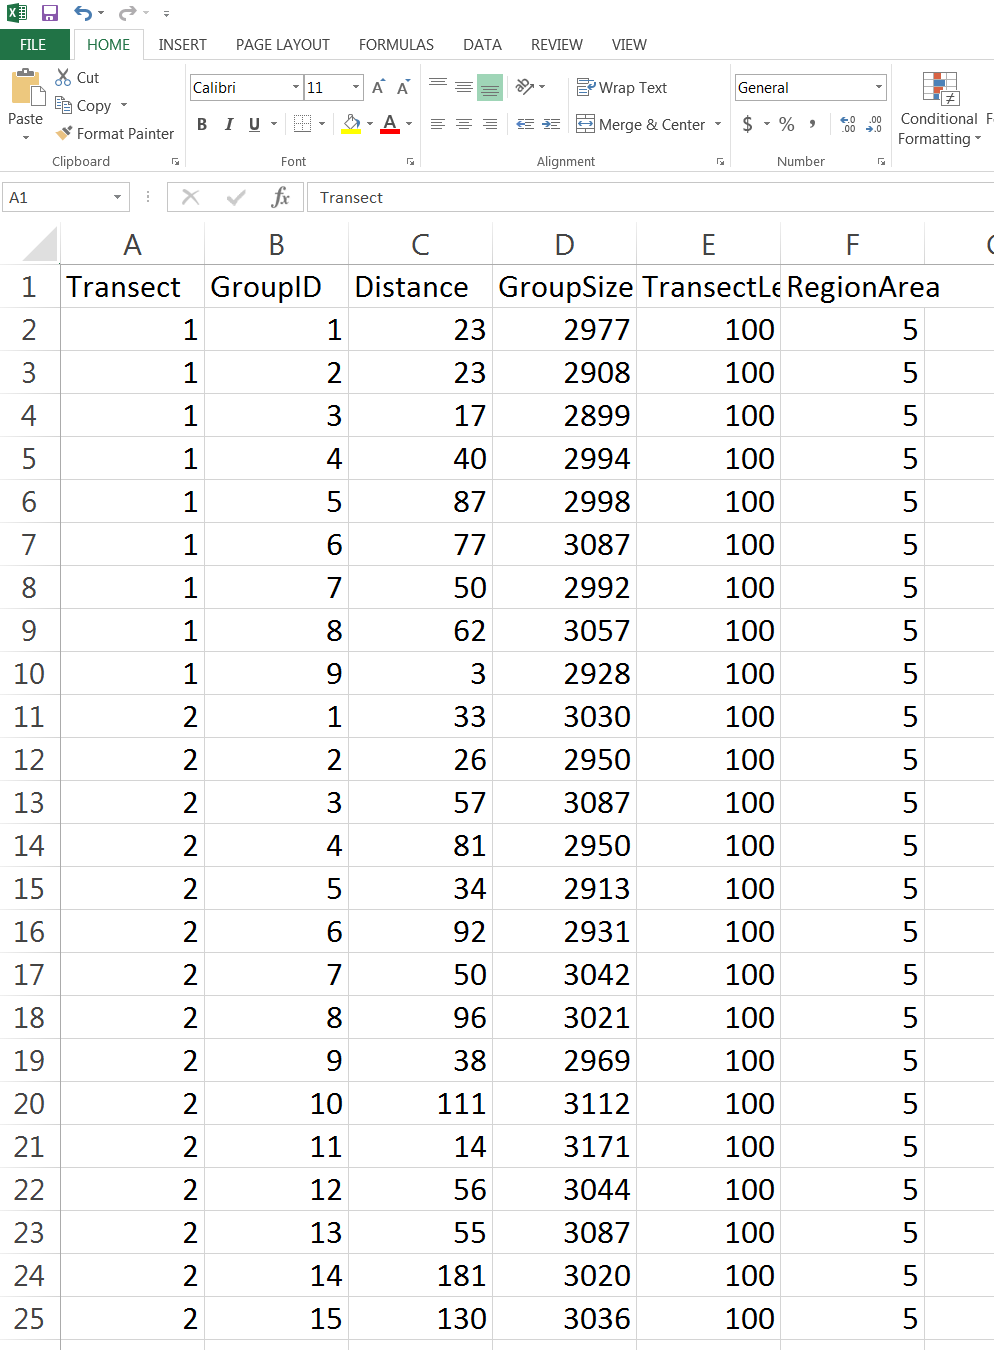
\includegraphics[height=8.5cm]{figs/ds-data1}} \hfill
  \fbox{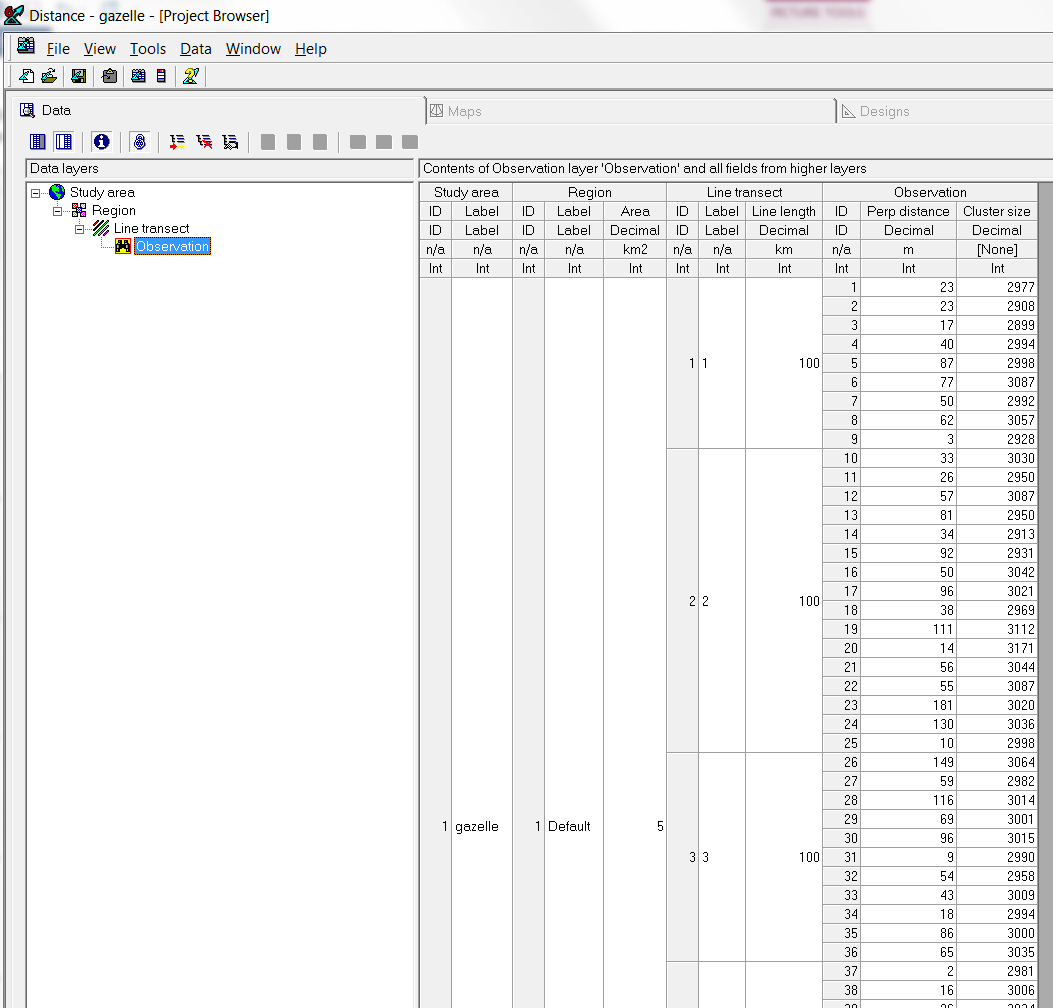
\includegraphics[height=8.5cm]{figs/ds-data2}}   \\
  \caption{\small Data formatted in Excel (left) and the same data in
    program DISTANCE.} 
  \label{fig:ds-data}
\end{figure}
%\clearpage



\clearpage

\section*{\large  Part II -- Estimate gazelle density and abundance}

\subsection*{\normalsize Half-normal detection function}


\begin{enumerate}
  \item Click the ``Analyses'' tab, then right click on the ``New 
    analysis'' line, and then choose ``Analysis details''.  
  \item Name this analysis ``Half-normal''
  \item Under ``data filters'', click on ``Properties'' and
    name the data filter ``truncate250''. Click on the ``Truncation''
    tab and tell it to discard all observations beyond 250m. Hit
    OK. 
  \item Under ``model definitions'' choose ``Properties'' and
    name it ``HN'' for half-normal. Then click the ``Detection
    function'' tab. Under ``Models'', specify a model with a
    half-normal ``key function''. Next, click on ``Adjustment terms''
    and choose ``Manual selection'' with 0 adjustment terms. Click the
    ``Cluster size'' tab and choose ``Use mean of observed
    clusters''. Hit ``OK''. 
  \item Run the model.
  \item On the ``Results'' tab on the right, scroll through the
    pages to the histograms of detection distances and the fitted
    detection function. Find the one that looks the best, in terms of
    the detection function fitting the histogram well, and then copy
    and paste it into your Word file. The easiest way to do this is to
    copy and paste into MS Paint and then save it as an image
    file. Then use \verb+Insert > Picture+ in Word.  Or you can take a
    screen shot of the histogram and paste that in. 
  \item Add a figure caption below the histogram that explains
    the graph.   
  \item Create a table to report estimates of abundance (N), density
    (D), group density (DS), sigma (called A(1) in DISTANCE), and
    p. Include standard errors (SEs) and confidence intervals (CIs) in
    your table. Define each of the parameters in your table (one sentence per parameter). 
\end{enumerate}


\subsection*{\normalsize Hazard-rate detection function}

\begin{enumerate}
  \item Run a second analysis in which you use a ``hazard-rate''
    detection function instead of the half-normal detection
    function. Do this by closing the results window, and
    right-clicking under the ``Analyses'' tab to select ``New Analysis\dots''.  
  \item Next, right-click on the new line that appeared (should be
    highlighted in blue) and choose `Analysis Details' again as you
    did before. Change the name of the analysis, and create a new
    `Model definition' in which you change the key function to
    `hazard-rate'. For all other options, use the same settings as
    before.   
  \item Repeat steps 6-7 above. Why do you think the results differ
    when you use different detection functions? Which of the two
    models is better (has the lower AIC)?  
\end{enumerate}



\end{document}




